% Some LaTeX commands I define for my own nomenclature.
% If you have to, it's better to change nomenclature once here than in a 
% million places throughout your thesis!



%======================================================================
\chapter{Objective 3: To explore patterns of information seeking and evacuation behaviors.}
\label{c6}

\section{Methodology}

For research objective 3, this study wanted to explore respondents' information-seeking behaviors and evacuation behaviors through their selections of behaviors. In order to understand which of the behaviors are preferred and which are selected more frequently, we chose to measure both the selected rate and the selected score. The calculation of the selected rate and the selected score will both do three times, for 300 Japanese samples, 1500 foreign visitors samples, and 1800 of all respondents' samples.

\subsection{Selected Rate}
Because the selected rate wants to explore which behaviors are used more, this part does not take the order factor into account. No matter the behavior is selected in which order, it will count as 1 point. The selected rate is equal to the Sum selected point divided by the sample number, shown in Figure~\ref{fig10}.

%%%%%%%%%%%%%%%%%%%%%%%%%%%%
%\iffalse
\begin{figure*}[h]
  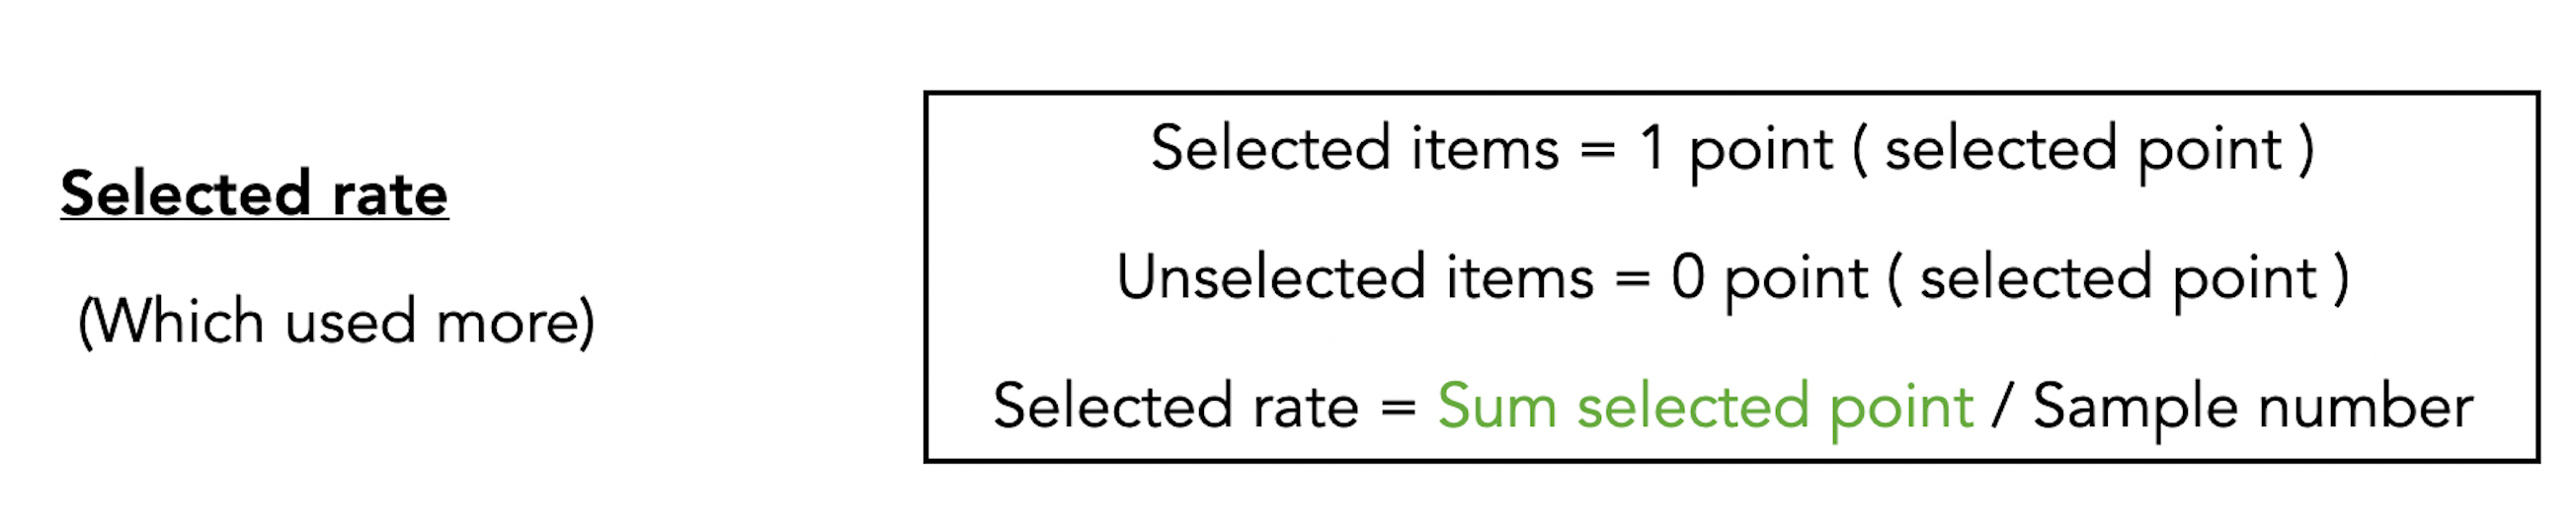
\includegraphics[width=\linewidth]{Figure/Figure10.png}
  \centering
  \caption{Selected rate }
  \label{fig10}
\end{figure*}
%\fi

\subsection{Selected Score}

Since the Selected score wants to explore which behaviors are used first, this part needs to take the order factor into account. The higher the preference is, the higher the score will be. So the first selected action is scored as 5, the second is scored as 4, the third is scored as 3, the fourth is scored as 2, and the last selected action is scored as 1. The Selected score is equal to the total score divided by the Sum selected point, shown in Figure~\ref{fig11}.

%%%%%%%%%%%%%%%%%%%%%%%%%%%
%\iffalse
\begin{figure*}[h]
  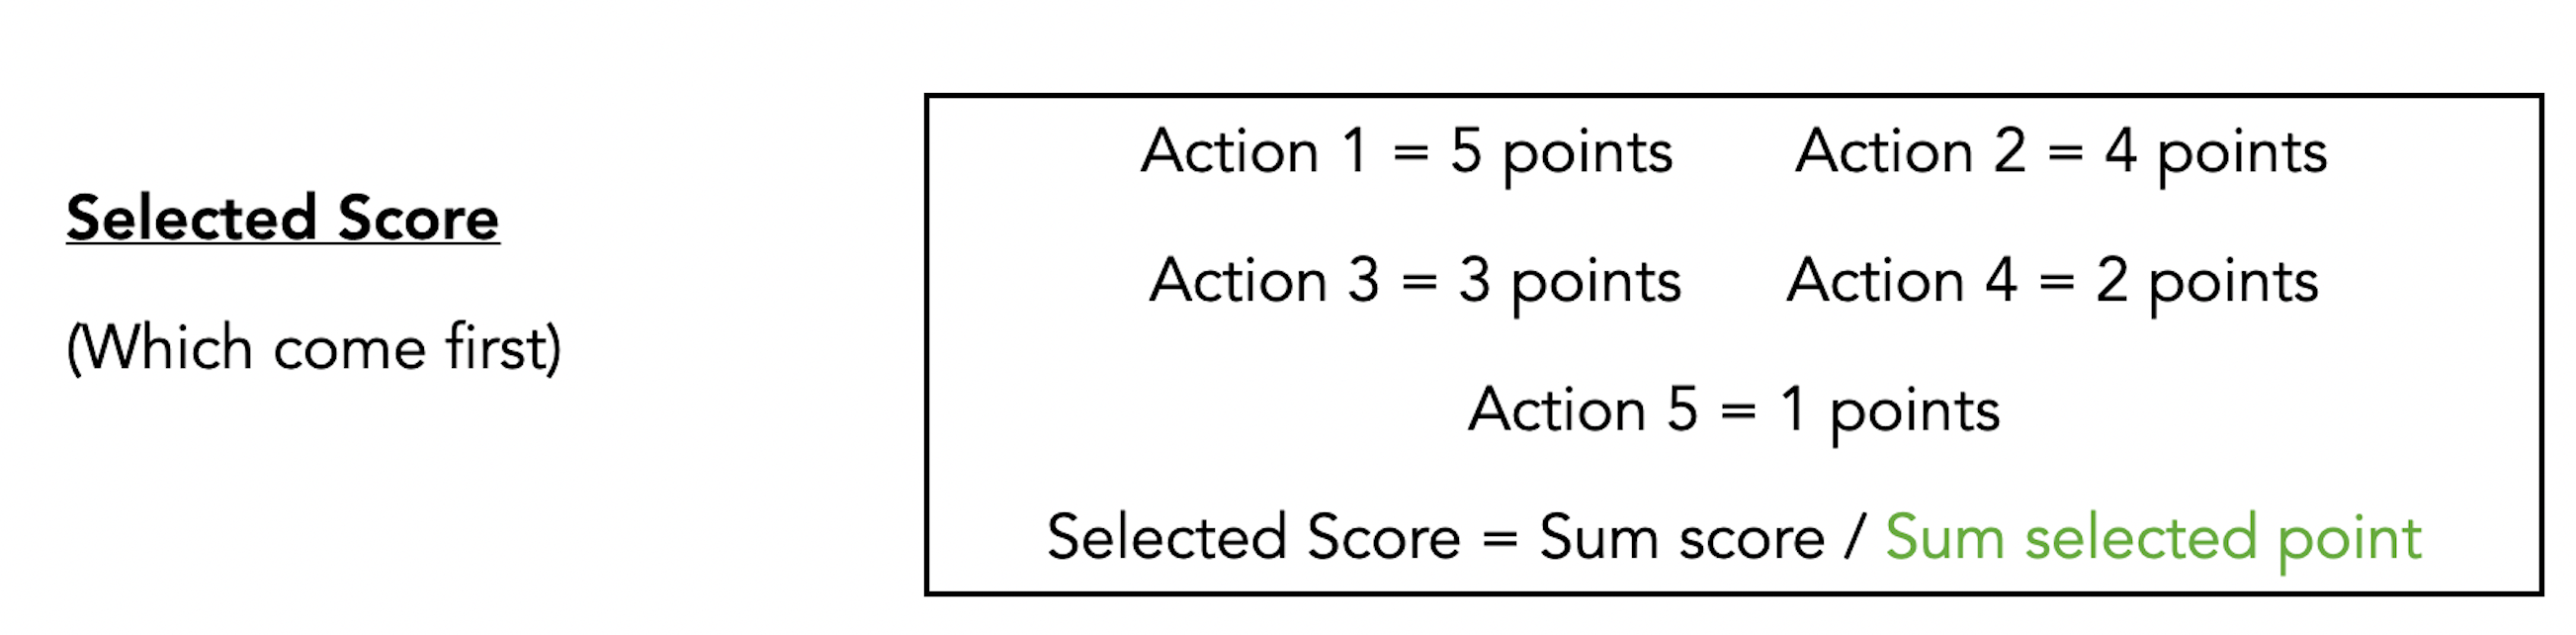
\includegraphics[width=\linewidth]{Figure/Figure11.png}
  \centering
  \caption{Selected score}
  \label{fig11}
\end{figure*}
%\fi

\subsection{Sankey Diagram of behavior patterns}

In the analysis of the selected score and selected rate of study objective 3, we will find that all the results will be relatively scattered. This is because, in this study, the number of available selections is relatively large, which makes the results more scattered. However, from the results, we can see that there could be similarities in the behavior patterns of people. Here the word 'pattern' means behavior patterns, not specific behavior. For example, the behavior of  'collecting information' is the same, the difference is how to collect information, from official websites, from disaster prevention software, from disaster prevention websites, from SNS, etc. So how to divide detailed behaviors into patterns? From the available selection, we can find that the behavior is mainly divided into two kinds, which are information-seeking behavior and evacuation behavior. First, regarding information-seeking behavior, we can find that there are two main patterns, one is 'No-face-to-face information seeking' and the other is 'Face-to-face information seeking'. And for the evacuation behavior, we can also find two main patterns, one is ' Self-evacuation behaviors ' and the other is ' Following evacuation guidance behavior '. Then, we divided all the selections into the patterns they belong to, which can be found in Figure~\ref{fig12}.

%%%%%%%%%%%%%%%%%%%%%%%%%%%
%\iffalse
\begin{figure*}[h]
  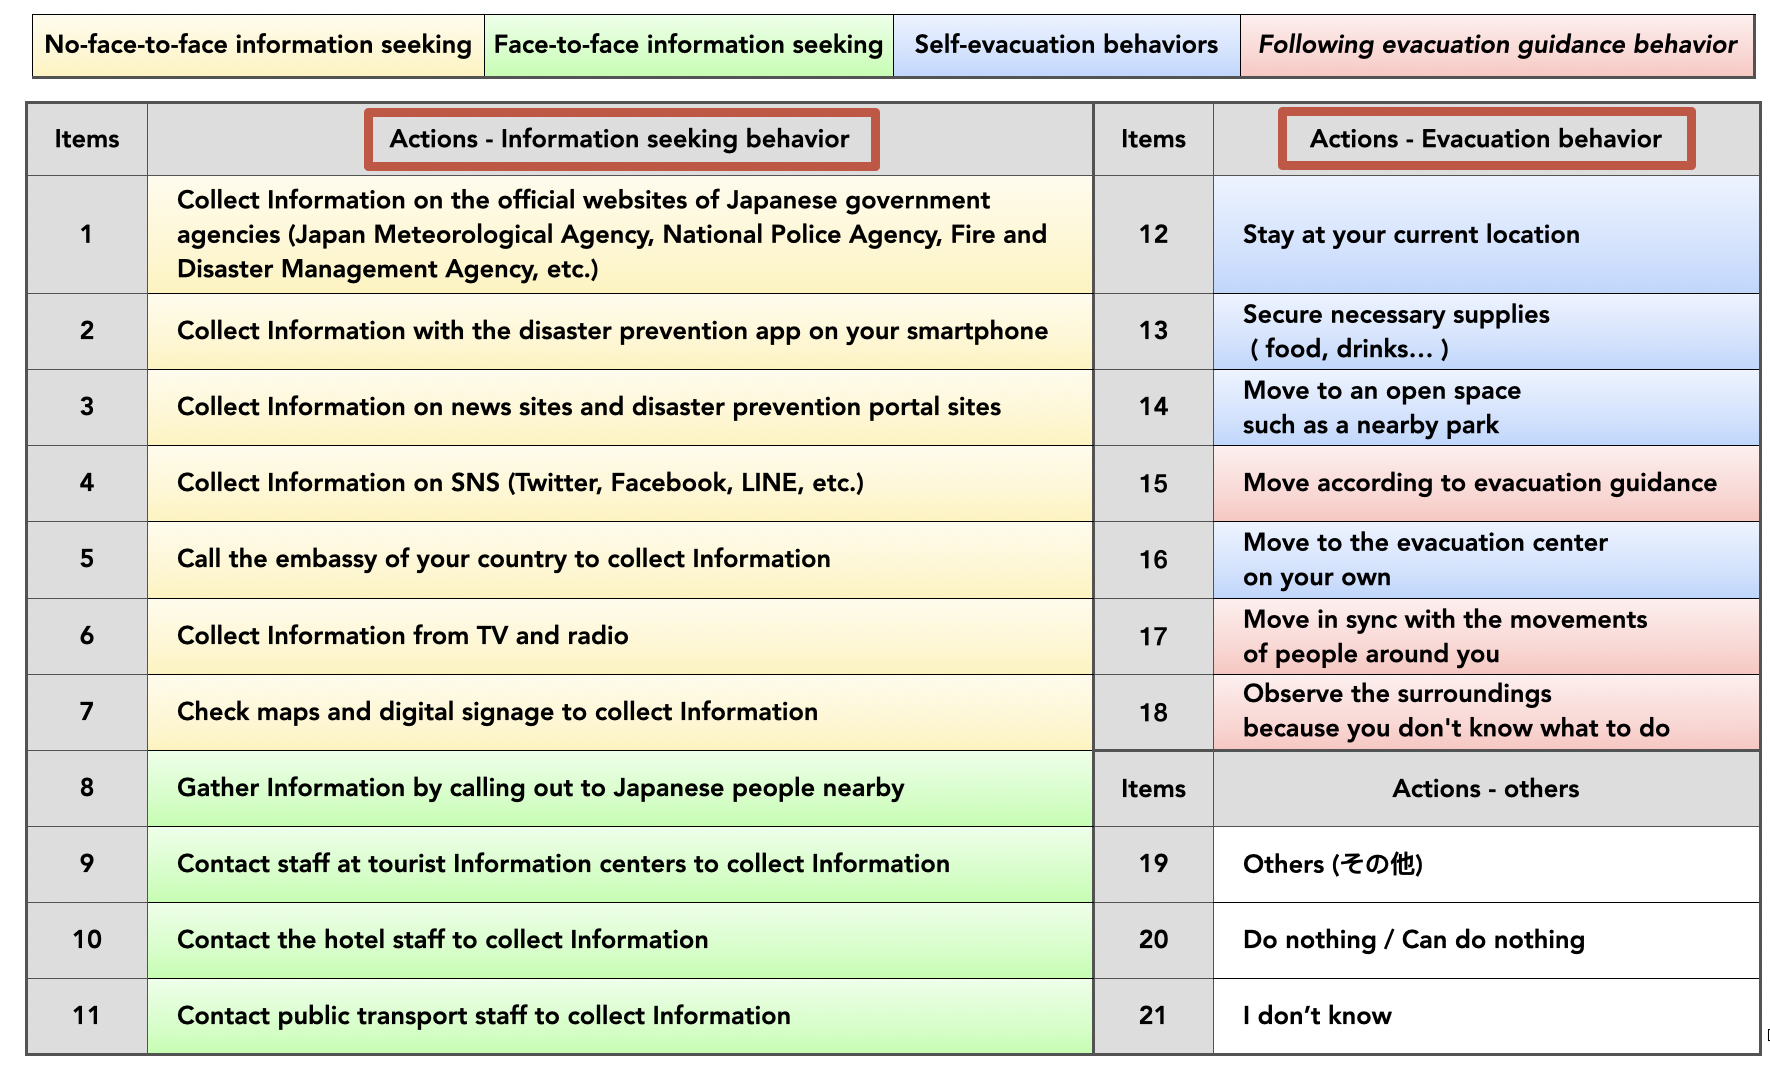
\includegraphics[width=\linewidth]{Figure/Figure12.png}
  \centering
  \caption{behavior patterns}
  \label{fig12}
\end{figure*}
%\fi

After attributing all the actions to the 4 patterns, we went through the flow of the respondents' actions with the help of the Sankey diagram. The Sankey diagram is a flow chart that shows the flow from each set of values to another set of values. The thickness of the lines expresses the number of values present in the group. In the Sankey diagram, the number indicates the No. of action, so 1-5 means the first action to the fifth action. Capital letters indicate behavior patterns.' No-face-to-face information seeking' is A; 'Face-to-face information seeking' is B; 'Self-evacuation behaviors' is C; 'Following evacuation guidance behavior' is D. Thus, the behavior from the first to the fifth cohort can be clearly represented in the results of the Sankey diagram. As an example, A1 indicates that the 1st response action during the disaster is behavior pattern A, which is 'No-face-to-face information seeking'.






\section{Result}


\subsection{Selected Score and Selected Rate}
The result of the Selected score and the Selected rate is shown in \crefrange{table17}{table20}. From the result, we can find that there are some differences between foreign visitors and Japanese in scenarios 1 and 3, which could show that when the internet and telephone are available, people tend to have various behaviors. By checking the Selected Rate, we can find that evacuation behaviors are more used than information-seeking behaviors. And among the evacuation behaviors, 'Moving according to evacuation guidance' could be used most. This indicates that, regardless of the order factor, 'Moving according to evacuation guidance' is the most favored option. In addition, people are more likely to heed evacuation instructions if they are in the area of such recommendations.  By checking the Selected Score, we can find that evacuation behaviors always happen before information-seeking behaviors. And among the evacuation behaviors, 'Observe the surroundings' could have happened first. This is compounded by the fact that many people's first instinct in the event of a disaster is to observe others. Not only might they receive some evacuation suggestions, but keeping the same pace as others will make people feel more at ease psychologically. 

Some lower used information-seeking behaviors during a disaster are 'Gather Information by calling out to Japanese people nearby', 'Contact staff at tourist Information centers to collect Information', 'Contact public transport staff to collect Information'. As a result, in the case of Internet\&Phone available, people do not choose to acquire information through methods that require verbal conversation, and instead prefer to obtain it on their own. On the other hand, because people can only obtain information through the verbal conversation when the Internet and phone are unavailable, their method of obtaining information depends on the scenario they are in. When people are in a tourist area, they usually ask Japanese people around them for information, and not many people choose the other three options of contacting staff at different spots. However, when people are moving by transportation, people still ask Japanese people around them for information, while contacting staff from public transportation is also a popular option. The lowest used evacuation behavior during a disaster is 'Stay at your current location. This is understandable after all, few people will just stay put and do nothing in the face of a disaster. It is important to note here that this result does not mean that everyone will necessarily do something to leave the place where it happened, but that people's priority evacuation behavior is less likely to be to stay where they are. People will, in most situations, choose to remain where they are after gathering information and following evacuation instructions. This section does not cover such circumstances.

%%%%%%%%%%%%%%%%%%%%%%%%%%
%\iffalse
\begin{table}[h]
  \caption[Result of Selected score and Selected rate in Scenario 1]{Result of Selected score and Selected rate in Scenario 1(No.: number of  selection, FV: Foreign Vistors, J: Japanese)}
  \label{table17}
  \centering 
  \begin{tabular}{cl|ccc|ccc}
                &   & \multicolumn{3}{c}{Selected Rate (\%)} & \multicolumn{3}{c}{Selected Score} \\
      No.     & \multicolumn{1}{c|}{Description} & All & FV & J & All & FV & J \\
 \hline
  1             & \begin{tabular}{l}Collect Information on the official websites\\of Japanese government agencies\end{tabular} & 31.6 &30.2 & 38.7 & 2.9 & 2.9 & 3.0 \\
  2             & \begin{tabular}{l}Collect Information with the disaster\\prevention app on your smartphone\end{tabular} & 27.9 & 25.4 & 40.7 & 2.9 & 2.8 & 3.2 \\
  3             & \begin{tabular}{l}Collect Information on news sites and\\disaster prevention portal sites\end{tabular} & 26.8 & 23.4 & 43.7 & 2.8 & 2.7 & 3.2 \\
  4             & \begin{tabular}{l}Collect Information on SNS\\(Twitter, Facebook, LINE, etc.)\end{tabular} & 19.9 & 18.2 & 28.7 & 2.8 & 2.7 & 3.0 \\
  5             & \begin{tabular}{l}Call the embassy of your country\\to collect Information\end{tabular} & 25.2 & 30.3 & N/A & 2.7 & 2.7 & N/A \\
  6             & \begin{tabular}{l}Collect Information from TV and radio\end{tabular} & 24.9 & 20.9 & 44.7 & 3.0 & 2.8 & 3.4 \\
  7             & \begin{tabular}{l}Check maps and digital signage to\\collect Information\end{tabular} & 14.4 & 15.0 & 11.7 & 2.8 & 2.8 & 2.9 \\
  8             & \begin{tabular}{l}Gather Information by calling out to\\Japanese people nearby\end{tabular} & 18.7 & 19.0 & 17.3 & 2.7 & 2.8 & 2.3 \\
  9             & \begin{tabular}{l}Contact staff at tourist Information\\centers to collect Information\end{tabular} & 16.0 & 18.3 & 4.3 & 2.9 & 2.9 & 2.3 \\
 10            & \begin{tabular}{l}Contact the hotel staff to collect\\Information\end{tabular} & 15.8 & 17.0 & 10.0 & 2.8 & 2.8 & 2.8 \\
 11            & \begin{tabular}{l}Contact public transport staff to\\collect Information\end{tabular} & 13.9 & 13.7 & 14.7 & 2.5 & 2.6 & 2.4 \\
 12            & \begin{tabular}{l}Stay at your current location\end{tabular} & 16.6 & 17.5 & 12.0 & 3.4 & 3.4 & 3.5 \\
 13            & \begin{tabular}{l}Secure necessary supplies\\(food, drink, etc.)\end{tabular}  & 32.9 & 33.0 & 32.3 & 3.0 & 3.1 & 2.8 \\
 14            & \begin{tabular}{l}Move to an open space such as a\\nearby park\end{tabular} & 39.7 & 41.8 & 29.0 & 3.3 & 3.3 & 3.0 \\
 15            & \begin{tabular}{l}Move according to evacuation\\guidance\end{tabular} & 53.7 & 54.9 & 47.7 & 3.4 & 3.5 & 3.2 \\
 16            & \begin{tabular}{l}Move to the evacuation center on\\your own\end{tabular} & 26.8 & 27.1 & 25.0 & 3.1 & 3.1 & 3.0 \\
 17            & \begin{tabular}{l}Move in sync with the movements\\of people around you\end{tabular} & 28.3 & 29.2 & 24.0 & 2.8 & 2.9 & 2.6 \\
 18            & \begin{tabular}{l}Observe the surroundings because\\you don't know what to do\end{tabular} & 45.2 & 44.7 & 48.0 & 3.6 & 3.6 & 3.4 \\
\hline
  \end{tabular}
\end{table}


\begin{table}[h]
  \caption[Result of Selected score and Selected rate in Scenario 2]{Result of Selected score and Selected rate in Scenario 2(No.: number of  selection, FV: Foreign Vistors, J: Japanese)}
  \label{table18}
  \centering 
  \begin{tabular}{cl|ccc|ccc}
                &   & \multicolumn{3}{c}{Selected Rate (\%)} & \multicolumn{3}{c}{Selected Score} \\
      No.     & \multicolumn{1}{c|}{Description} & All & FV & J & All & FV & J \\
 \hline
  8             & \begin{tabular}{l}Gather Information by calling out to\\Japanese people nearby\end{tabular} & 41.1 & 40.5 & 44.0 & 2.8 & 2.8 & 2.9 \\
  9             & \begin{tabular}{l}Contact staff at tourist Information\\centers to collect Information\end{tabular} & 33.8 & 36.8 & 18.7 & 2.7 & 2.7 & 2.4 \\
 10            & \begin{tabular}{l}Contact the hotel staff to collect\\Information\end{tabular} & 33.0 & 34.3 & 26.7 & 2.9 & 2.8 & 3.0 \\
 11            & \begin{tabular}{l}Contact public transport staff to\\collect Information\end{tabular} & 29.8 & 29.3 & 32.7 & 2.7 & 2.6 & 2.8 \\
 12            & \begin{tabular}{l}Stay at your current location\end{tabular} & 23.9 & 24.7 & 20.0 & 3.0 & 3.0 & 3.0 \\
 13            & \begin{tabular}{l}Secure necessary supplies\\(food, drink, etc.)\end{tabular}  & 44.5 & 44.4 & 45.0 & 2.9 & 2.9 & 3.0 \\
 14            & \begin{tabular}{l}Move to an open space such as a\\nearby park\end{tabular} & 52.5 & 54.5 & 44.7 & 3.2 & 3.2 & 3.1 \\
 15            & \begin{tabular}{l}Move according to evacuation\\guidance\end{tabular} & 66.6 & 65.9 & 70.0 & 3.4 & 3.4 & 3.5 \\
 16            & \begin{tabular}{l}Move to the evacuation center on\\your own\end{tabular} & 39.3 & 37.9 & 46.3 & 2.9 & 2.9 & 2.7 \\
 17            & \begin{tabular}{l}Move in sync with the movements\\of people around you\end{tabular} & 46.5 & 47.3 & 42.7 & 2.9 & 3.0 & 2.8 \\
 18            & \begin{tabular}{l}Observe the surroundings because\\you don't know what to do\end{tabular} & 61.6 & 60.7 & 66.0 & 3.6 & 3.5 & 3.8 \\
\hline
  \end{tabular}
\end{table}



\begin{table}[h]
  \caption[Result of Selected score and Selected rate in Scenario 3]{Result of Selected score and Selected rate in Scenario 3(No.: number of  selection, FV: Foreign Vistors, J: Japanese)}
  \label{table19}
  \centering 
  \begin{tabular}{cl|ccc|ccc}
                &   & \multicolumn{3}{c}{Selected Rate (\%)} & \multicolumn{3}{c}{Selected Score} \\
      No.     & \multicolumn{1}{c|}{Description} & All & FV & J & All & FV & J \\
 \hline
  1             & \begin{tabular}{l}Collect Information on the official websites\\of Japanese government agencies\end{tabular} & 29.1 & 28.6 & 31.1 & 3.0 & 3.0 & 3.0 \\
  2             & \begin{tabular}{l}Collect Information with the disaster\\prevention app on your smartphone\end{tabular} & 29.4 & 27.1 & 41.0 & 3.0 & 2.9 & 3.2 \\
  3             & \begin{tabular}{l}Collect Information on news sites and\\disaster prevention portal sites\end{tabular} & 27.6 & 24.5 & 43.0 & 2.8 & 2.7 & 3.2 \\
  4             & \begin{tabular}{l}Collect Information on SNS\\(Twitter, Facebook, LINE, etc.)\end{tabular} & 24.6 & 22.7 & 34.3 & 2.8 & 2.7 & 3.0 \\
  5             & \begin{tabular}{l}Call the embassy of your country\\to collect Information\end{tabular} & 24.2 & 29.0 & N/A & 2.9 & 2.9 & N/A \\
  6             & \begin{tabular}{l}Collect Information from TV and radio\end{tabular} & 22.4 & 19.3 & 37.7 & 2.9 & 2.8 & 3.0 \\
  7             & \begin{tabular}{l}Check maps and digital signage to\\collect Information\end{tabular} & 15.7 & 16.2 & 13.3 & 2.9 & 2.9 & 2.9 \\
  8             & \begin{tabular}{l}Gather Information by calling out to\\Japanese people nearby\end{tabular} & 20.7 & 21.1 & 18.3 & 2.7 & 2.7 & 2.7 \\
  9             & \begin{tabular}{l}Contact staff at tourist Information\\centers to collect Information\end{tabular} & 16.8 & 18.8 & 7.0 & 2.7 & 2.7 & 2.7 \\
 10            & \begin{tabular}{l}Contact the hotel staff to collect\\Information\end{tabular} & 15.4 & 17.1 & 7.0 & 2.8 & 2.8 & 2.9 \\
 11            & \begin{tabular}{l}Contact public transport staff to\\collect Information\end{tabular} & 23.9 & 22.6 & 30.7 & 3.0 & 3.0 & 3.1 \\
 12            & \begin{tabular}{l}Stay at your current location\end{tabular} & 13.7 & 14.3 & 10.3 & 3.6 & 3.7 & 2.9 \\
 13            & \begin{tabular}{l}Secure necessary supplies\\(food, drink, etc.)\end{tabular}  & 27.8 & 28.3 & 25.3 & 3.0 & 3.0 & 2.9 \\
 14            & \begin{tabular}{l}Move to an open space such as a\\nearby park\end{tabular} & 34.6 & 37.6 & 19.3 & 3.2 & 3.2 & 2.9 \\
 15            & \begin{tabular}{l}Move according to evacuation\\guidance\end{tabular} & 50.7 & 50.9 & 50.0 & 3.4 & 3.4 & 3.2 \\
 16            & \begin{tabular}{l}Move to the evacuation center on\\your own\end{tabular} & 26.6 & 27.9 & 20.3 & 2.9 & 2.9 & 2.8 \\
 17            & \begin{tabular}{l}Move in sync with the movements\\of people around you\end{tabular} & 32.4 & 33.6 & 26.7 & 2.9 & 2.9 & 2.8 \\
 18            & \begin{tabular}{l}Observe the surroundings because\\you don't know what to do\end{tabular} & 41.1 & 40.8 & 42.7 & 3.7 & 3.7 & 3.5 \\
\hline
  \end{tabular}
\end{table}


\begin{table}[h]
  \caption[Result of Selected score and Selected rate in Scenario 4]{Result of Selected score and Selected rate in Scenario 4(No.: number of  selection, FV: Foreign Vistors, J: Japanese)}
  \label{table20}
  \centering 
  \begin{tabular}{cl|ccc|ccc}
                &   & \multicolumn{3}{c}{Selected Rate (\%)} & \multicolumn{3}{c}{Selected Score} \\
      No.     & \multicolumn{1}{c|}{Description} & All & FV & J & All & FV & J \\
 \hline
  8             & \begin{tabular}{l}Gather Information by calling out to\\Japanese people nearby\end{tabular} & 42.3 & 43.4 & 37.0 & 2.8 & 2.8 & 2.8 \\
  9             & \begin{tabular}{l}Contact staff at tourist Information\\centers to collect Information\end{tabular} & 29.2 & 32.1 & 14.7 & 2.7 & 2.7 & 2.7 \\
 10            & \begin{tabular}{l}Contact the hotel staff to collect\\Information\end{tabular} & 27.2 & 29.5 & 15.7 & 2.9 & 2.9 & 2.8 \\
 11            & \begin{tabular}{l}Contact public transport staff to\\collect Information\end{tabular} & 40.9 & 39.4 & 48.3 & 3.1 & 3.0 & 3.4 \\
 12            & \begin{tabular}{l}Stay at your current location\end{tabular} & 24.3 & 24.8 & 21.7 & 3.1 & 3.2 & 3.0 \\
 13            & \begin{tabular}{l}Secure necessary supplies\\(food, drink, etc.)\end{tabular}  & 39.1 & 39.2 & 38.3 & 2.8 & 2.9 & 2.8 \\
 14            & \begin{tabular}{l}Move to an open space such as a\\nearby park\end{tabular} & 49.8 & 52.2 & 37.7 & 3.0 & 3.0 & 2.6 \\
 15            & \begin{tabular}{l}Move according to evacuation\\guidance\end{tabular} & 67.7 & 66.2 & 75.0 & 3.5 & 3.4 & 3.6 \\
 16            & \begin{tabular}{l}Move to the evacuation center on\\your own\end{tabular} & 41.1 & 40.9 & 42.0 & 2.8 & 2.8 & 2.5 \\
 17            & \begin{tabular}{l}Move in sync with the movements\\of people around you\end{tabular} & 50.6 & 50.9 & 49.0 & 2.9 & 3.0 & 2.8 \\
 18            & \begin{tabular}{l}Observe the surroundings because\\you don't know what to do\end{tabular} & 59.2 & 57.5 & 67.7 & 3.5 & 3.5 & 3.6 \\
\hline
  \end{tabular}
\end{table}
%\fi
\cleardoublepage
\subsection{Sankey Diagram of behavior patterns}

Figure~\ref{fig26} depicts the Sankey Diagram for foreign visitors in scenarios 1 to 4, whereas Figure~\ref{fig27} depicts the Sankey Diagram for Japanese visitors in scenarios 1 to 4. Figure~\ref{fig28} shows a summary of the Sankey Diagram data, with blue denoting the action with the highest value. 

\begin{figure*}[h]
  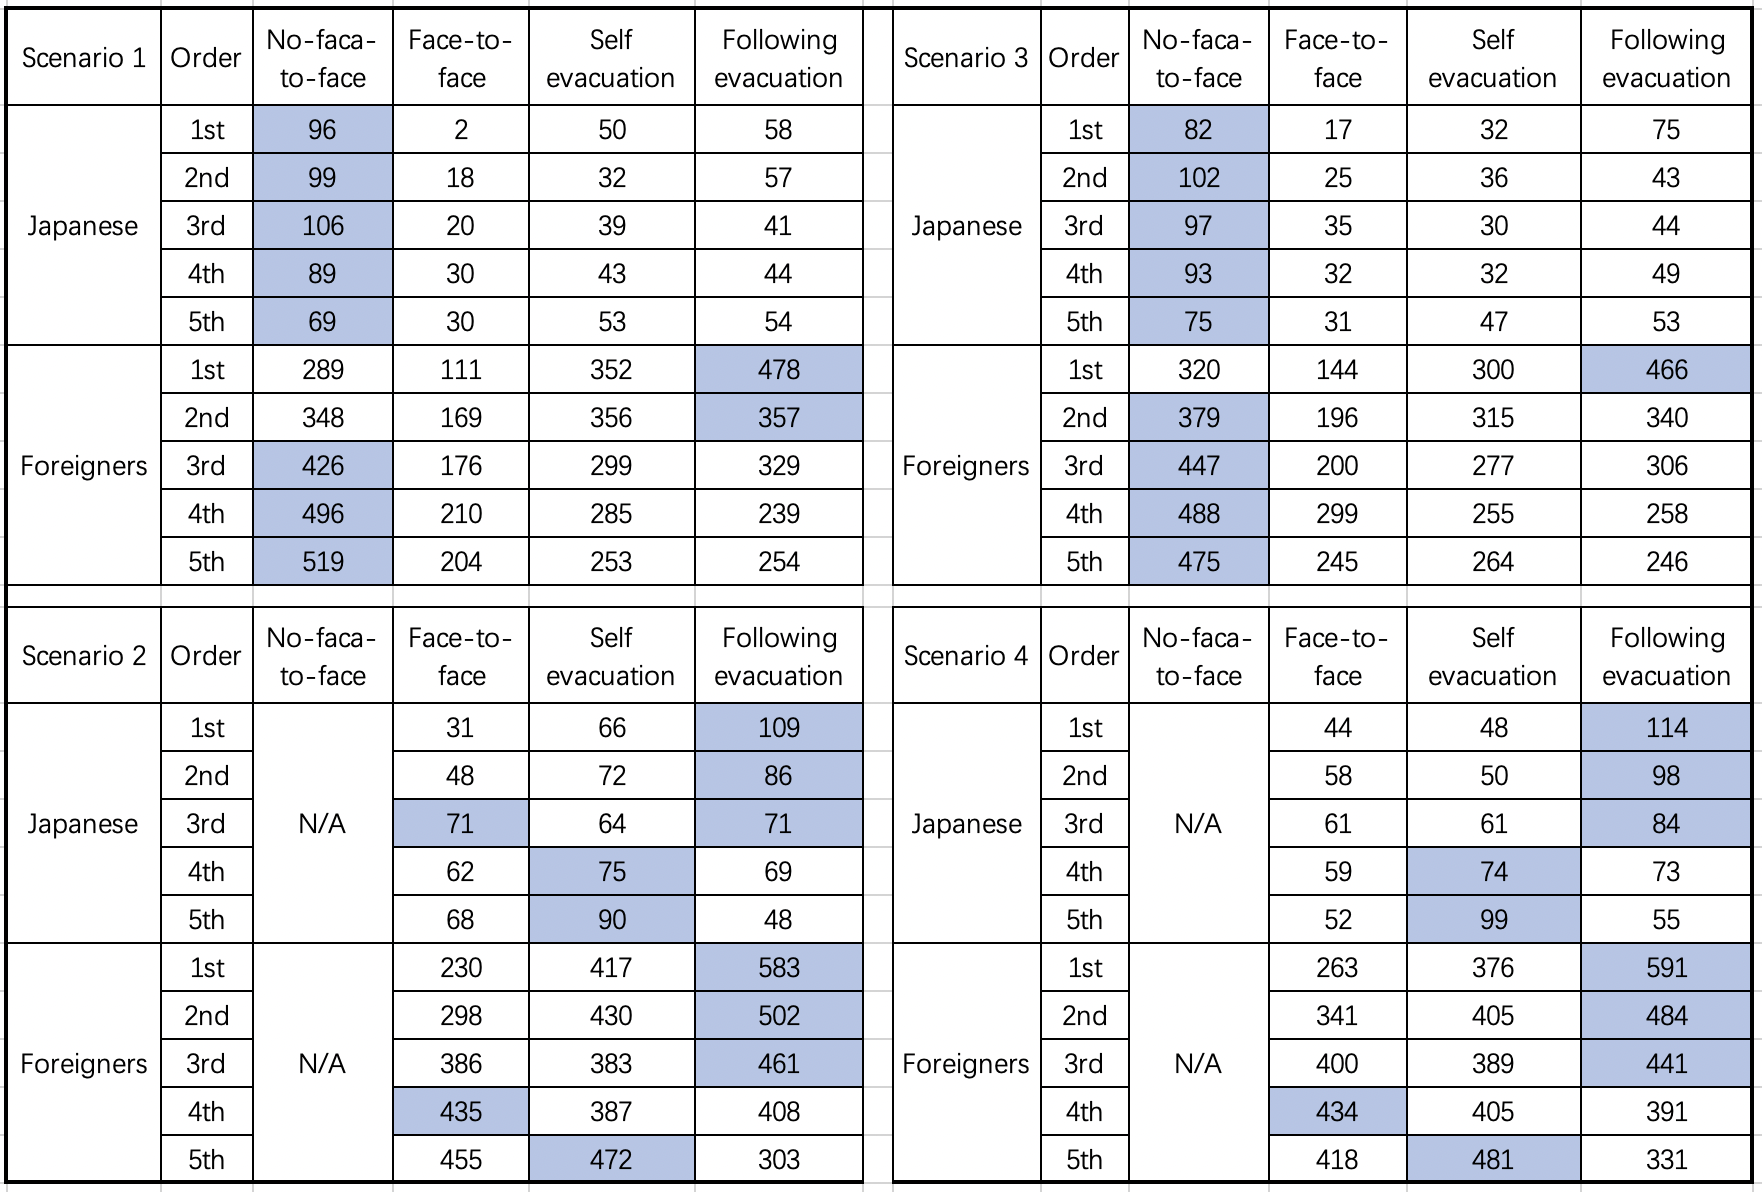
\includegraphics[width=\linewidth]{Figure/Figure28.jpg}
  \centering
  \caption{Summary of Sankey diagram data}
  \label{fig28}
\end{figure*}

%%%%%%%%%%%%%%%%%%%%%%%%%%
%\iffalse
\begin{figure*}[h]
  \begin{subfigure}{0.5\textwidth}
    \centering
    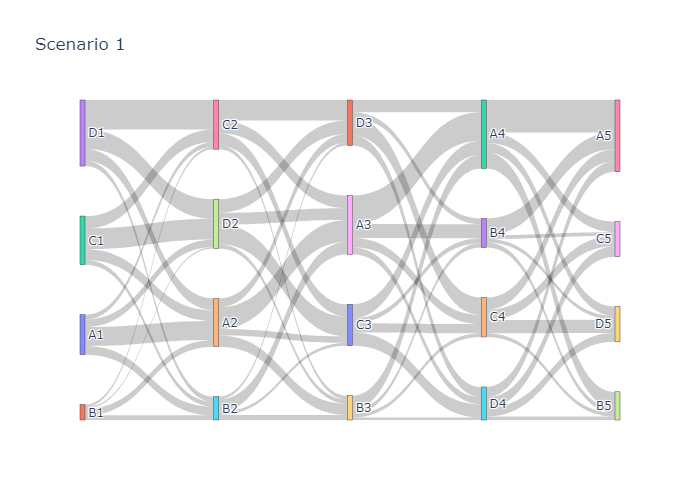
\includegraphics[width=\textwidth]{Figure/Figure26a.jpg}
    \caption{In scenario 1}
    \label{fig26a}
  \end{subfigure}
  \begin{subfigure}{0.5\textwidth}
    \centering
    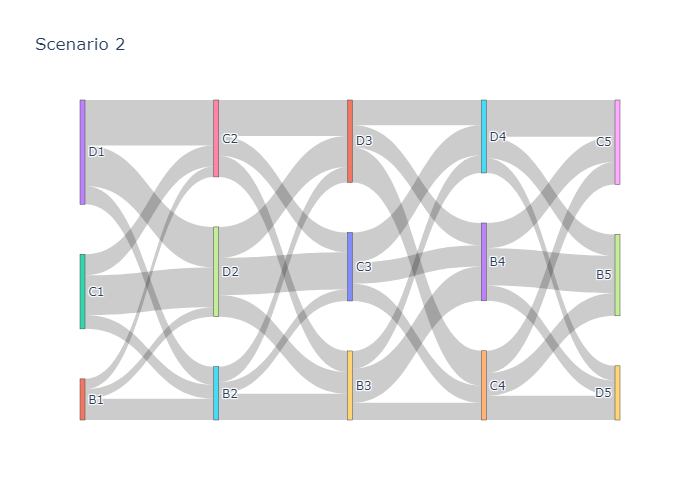
\includegraphics[width=\linewidth]{Figure/Figure26b.jpg}
    \caption{In scenario 2}
    \label{fig26b}
  \end{subfigure}
  \begin{subfigure}{0.5\textwidth}
    \centering
    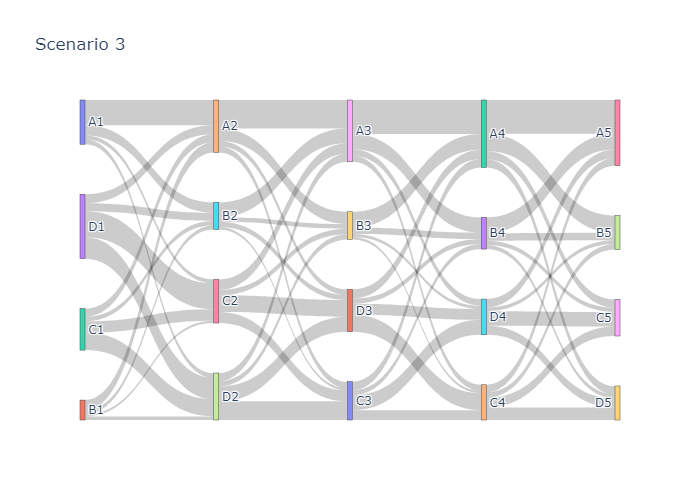
\includegraphics[width=\linewidth]{Figure/Figure26c.jpg}
    \caption{In scenario 3}
    \label{fig26c}
  \end{subfigure}
  \begin{subfigure}{0.5\textwidth}
    \centering
    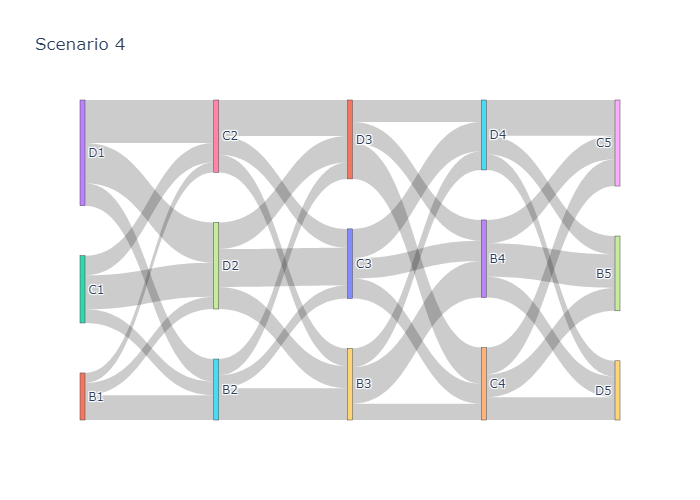
\includegraphics[width=\linewidth]{Figure/Figure26d.jpg}
    \caption{In scenario 4}
    \label{fig26d}
  \end{subfigure}
  \caption{Sankey diagram of foreign visitors }
  \label{fig26}
\end{figure*}

\begin{figure*}[h]
  \begin{subfigure}{0.5\textwidth}
    \centering
    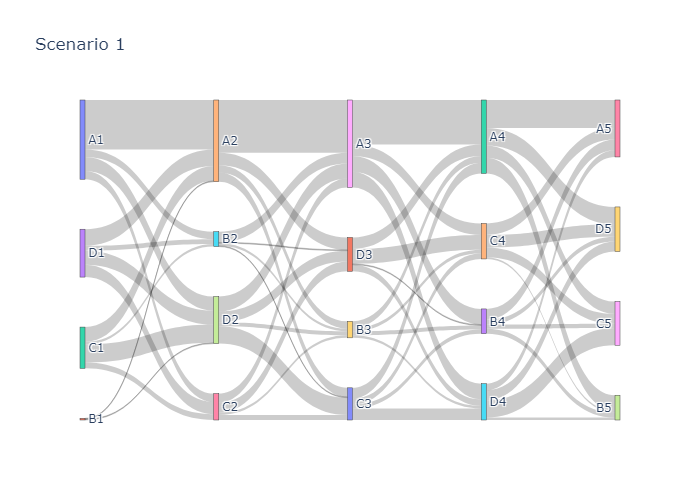
\includegraphics[width=\textwidth]{Figure/Figure27a.jpg}
    \caption{In scenario 1}
    \label{fig27a}
  \end{subfigure}
  \begin{subfigure}{0.5\textwidth}
    \centering
    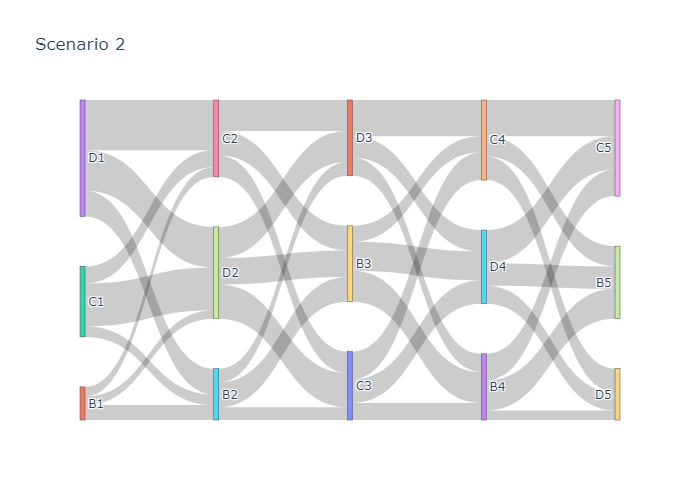
\includegraphics[width=\linewidth]{Figure/Figure27b.jpg}
    \caption{In scenario 2}
    \label{fig27b}
  \end{subfigure}
  \begin{subfigure}{0.5\textwidth}
    \centering
    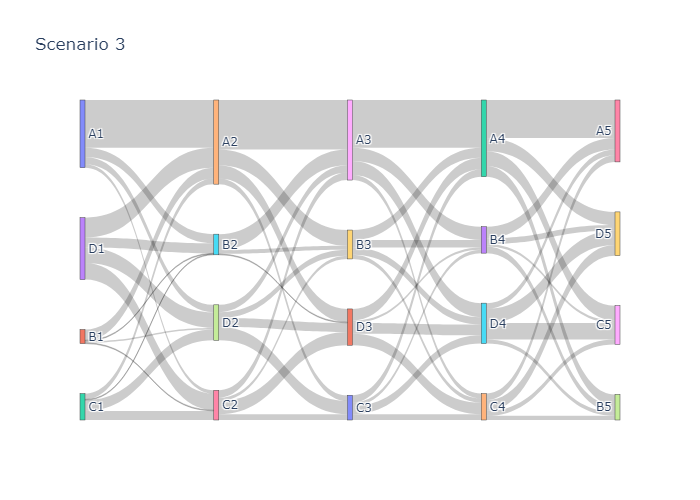
\includegraphics[width=\linewidth]{Figure/Figure27c.jpg}
    \caption{In scenario 3}
    \label{fig27c}
  \end{subfigure}
  \begin{subfigure}{0.5\textwidth}
    \centering
    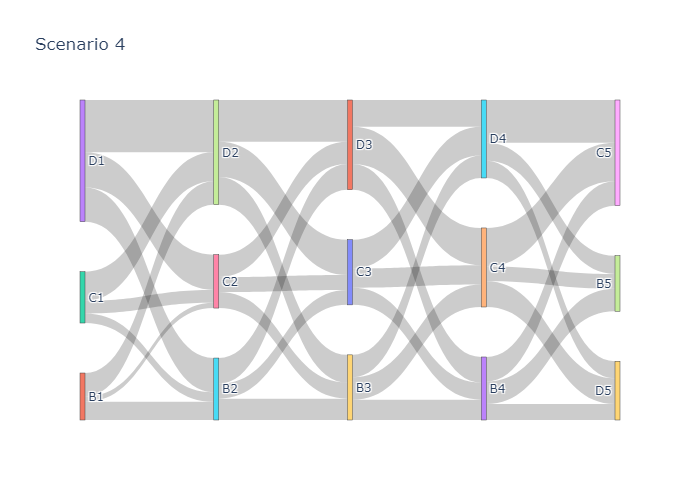
\includegraphics[width=\linewidth]{Figure/Figure27d.jpg}
    \caption{In scenario 4}
    \label{fig27d}
  \end{subfigure}
  \caption{Sankey diagram of Japanese }
  \label{fig27}
\end{figure*}


%\fi

We can learn from the data that No-face-to-face information seeking is more common than face-to-face information seeking. In the top three actions, following evacuation guidance behaviors are more common than self-evacuation behaviors. 

On the other hand, when the internet and telephone are available, Japanese prefer to take No-face-to-face information-seeking behaviors, while foreign visitors prefer to take following evacuation guidance behavior first, then trend to take No-face-to-face information-seeking behaviors. 

When the internet and phone are unavailable, both Japanese and foreign visitors show similar behavior. Both Japanese and foreigners prefer to take following evacuation guidance behaviors first. However, there are some differences in the behaviors that followed. Self-evacuation behaviors are preferred by the Japanese, while foreigners prefer face-to-face information-seeking behaviors before self-evacuation behaviors.

We can more clearly see the differences between foreign visitors and Japanese when we attribute specific actions to behavior patterns. The most common actions among Japanese in scenarios 1 and 3 are all No-face-to-face information seeking, but the most common behaviors among foreign tourists are following evacuation guidance behaviors, followed by No-face-to-face information seeking. 

I also used the Sankey diagram to analyze the flow of respondents' response actions in each country. The results are shown in \crefrange{fig32}{fig35}. But from the graph we can actually hardly see the difference, basically, the action selection is similar in terms of ratio for each cis. This proves that there is little variability among foreigners and people's actions are not influenced by differences in home country nationality.



\begin{figure*}[h]
  \begin{subfigure}{0.5\textwidth}
    \centering
    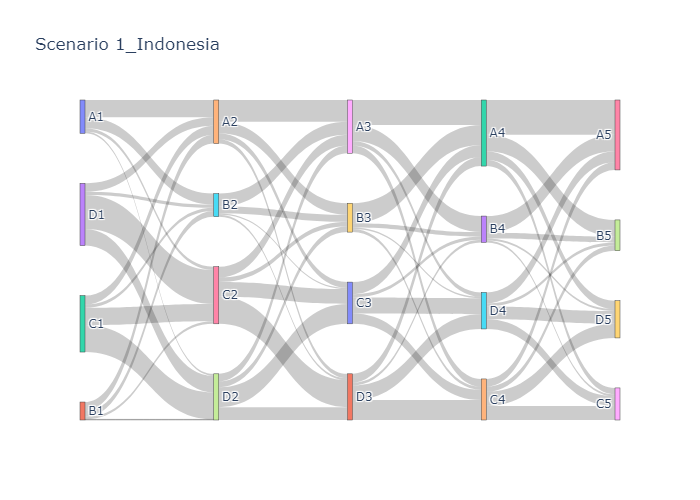
\includegraphics[width=\textwidth]{Figure/figure32a.png}
    \caption{Indonesia}
  \end{subfigure}
  \begin{subfigure}{0.5\textwidth}
    \centering
    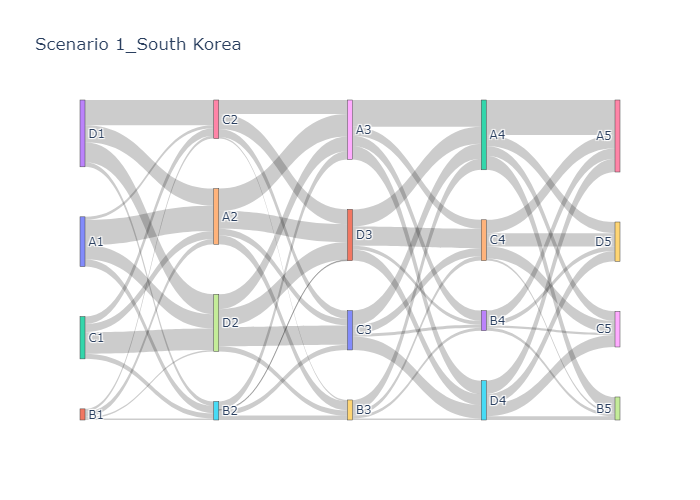
\includegraphics[width=\linewidth]{Figure/figure33a.png}
    \caption{South Korea}
  \end{subfigure}
  \begin{subfigure}{0.5\textwidth}
    \centering
    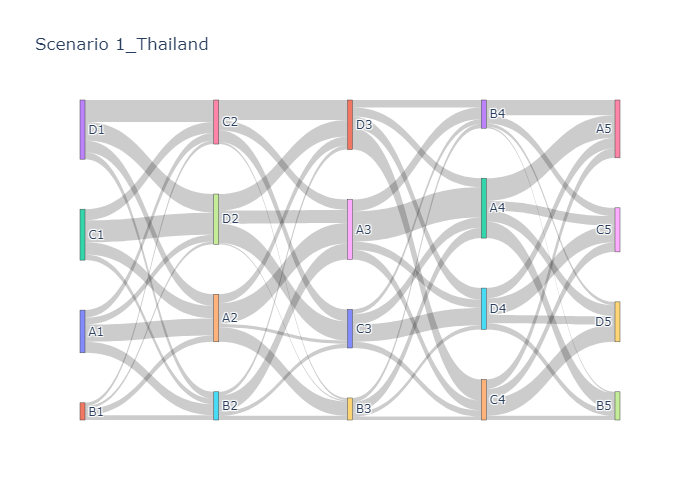
\includegraphics[width=\linewidth]{Figure/figure34a.png}
    \caption{Thailand}
  \end{subfigure}
  \begin{subfigure}{0.5\textwidth}
    \centering
    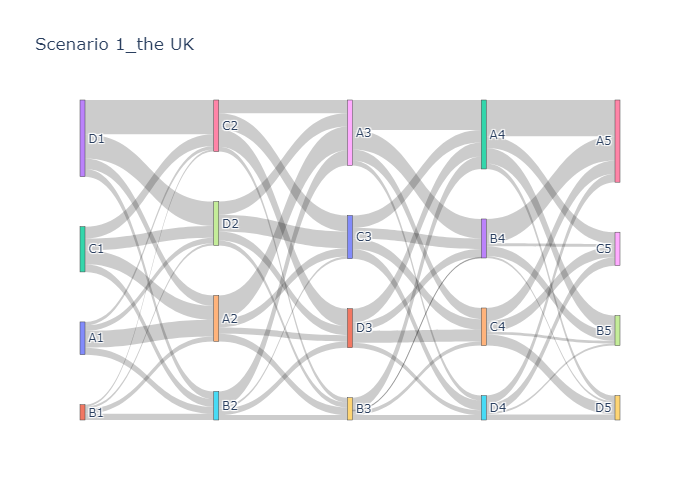
\includegraphics[width=\linewidth]{Figure/figure35a.png}
    \caption{the UK}
  \end{subfigure}
  \begin{subfigure}{0.5\textwidth}
    \centering
    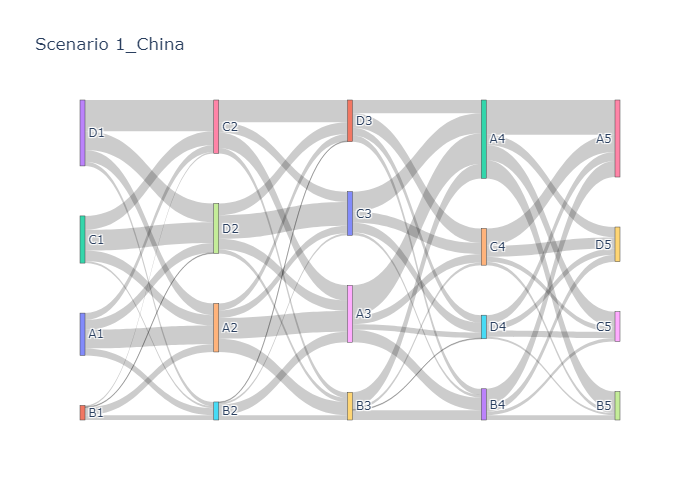
\includegraphics[width=\linewidth]{Figure/figure36a.png}
    \caption{China}
  \end{subfigure}
  \caption{ Sankey diagram of foreign vistors in senario 1 }
  \label{fig32}
\end{figure*}

\begin{figure*}[h]
  \begin{subfigure}{0.5\textwidth}
    \centering
    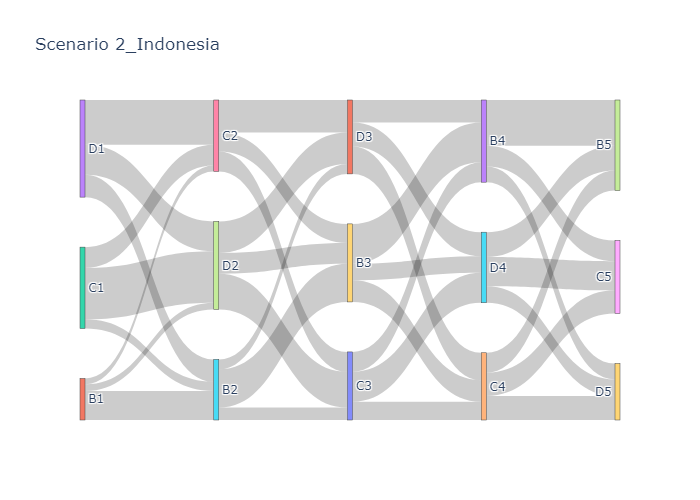
\includegraphics[width=\textwidth]{Figure/figure32b.png}
    \caption{Indonesia}
  \end{subfigure}
  \begin{subfigure}{0.5\textwidth}
    \centering
    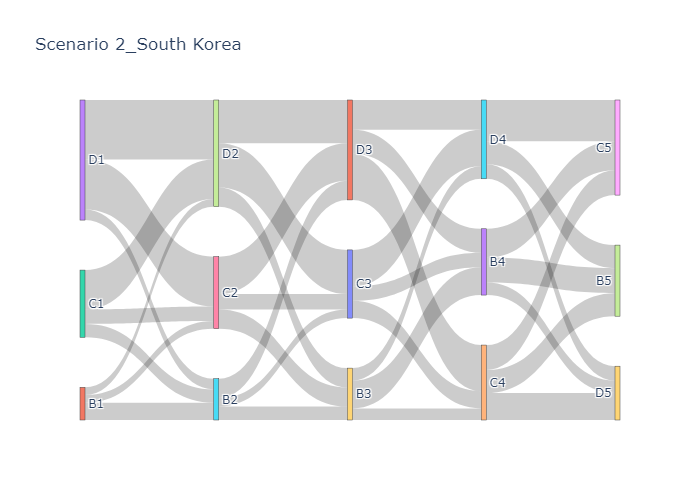
\includegraphics[width=\linewidth]{Figure/figure33b.png}
    \caption{South Korea}
  \end{subfigure}
  \begin{subfigure}{0.5\textwidth}
    \centering
    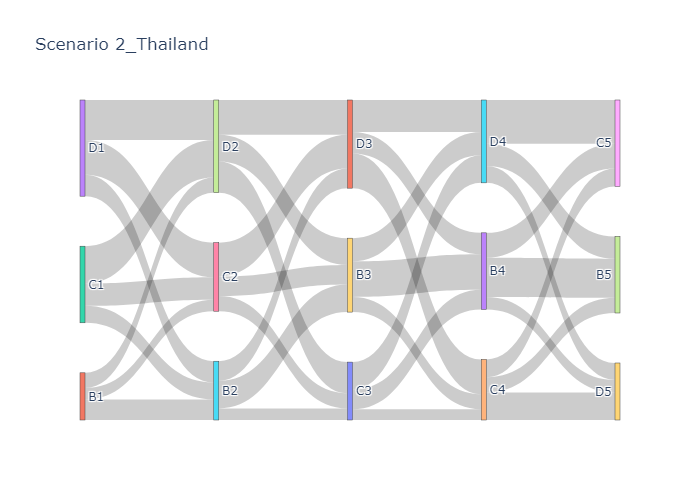
\includegraphics[width=\linewidth]{Figure/figure34b.png}
    \caption{Thailand}
  \end{subfigure}
  \begin{subfigure}{0.5\textwidth}
    \centering
    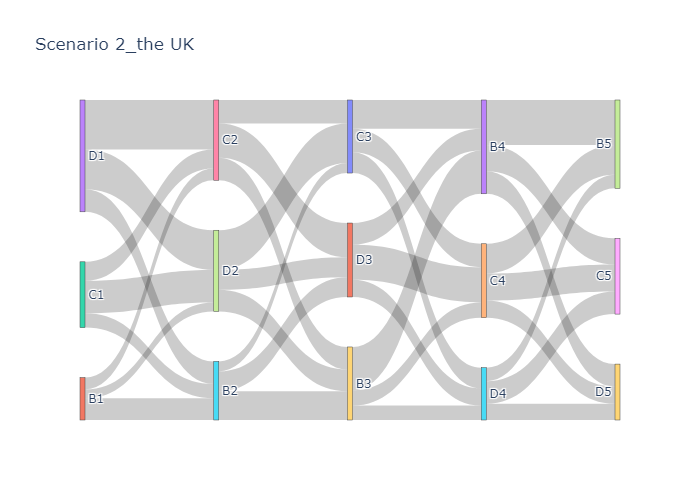
\includegraphics[width=\linewidth]{Figure/figure35b.png}
    \caption{the UK}
  \end{subfigure}
  \begin{subfigure}{0.5\textwidth}
    \centering
    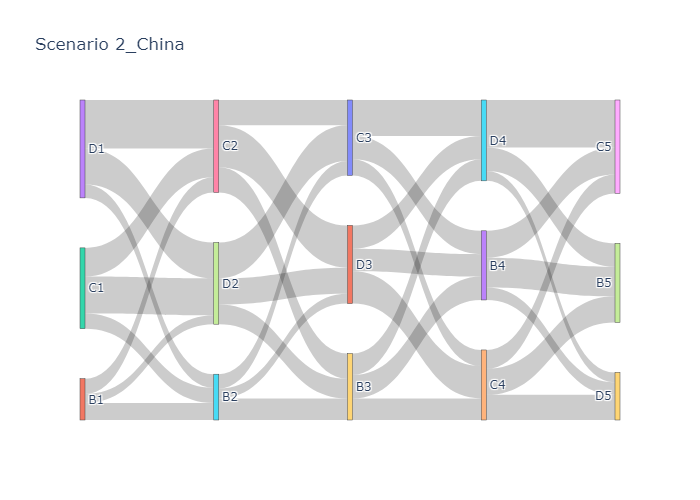
\includegraphics[width=\linewidth]{Figure/figure36b.png}
    \caption{China}
  \end{subfigure}
  \caption{ Sankey diagram of foreign vistors in senario 2 }
  \label{fig33}
\end{figure*}

\begin{figure*}[h]
  \begin{subfigure}{0.5\textwidth}
    \centering
    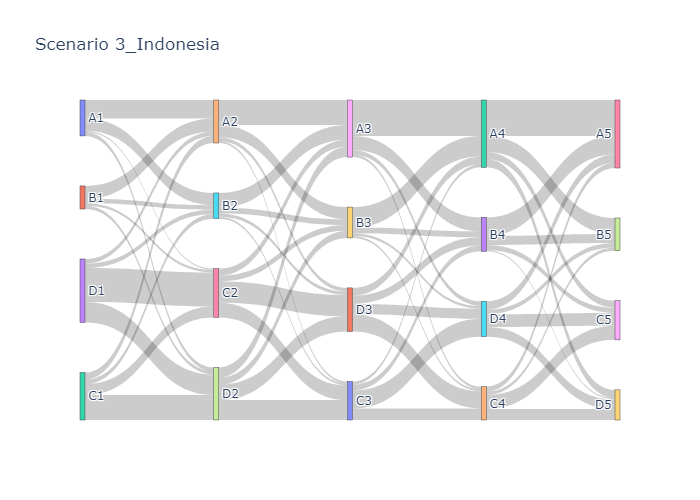
\includegraphics[width=\textwidth]{Figure/figure32c.png}
    \caption{Indonesia}
  \end{subfigure}
  \begin{subfigure}{0.5\textwidth}
    \centering
    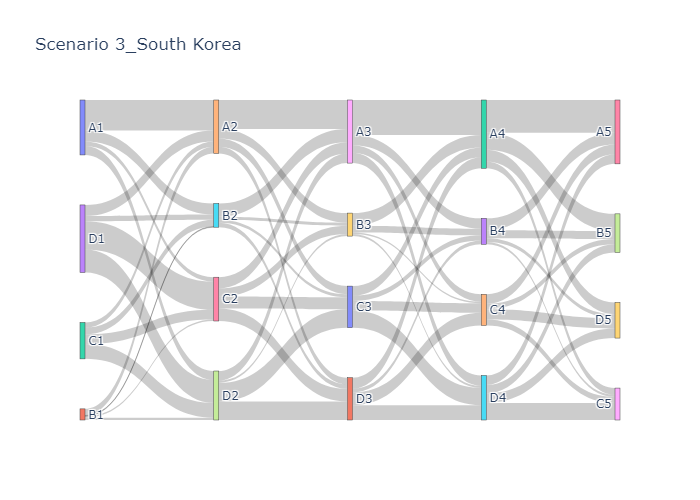
\includegraphics[width=\linewidth]{Figure/figure33c.png}
    \caption{South Korea}
  \end{subfigure}
  \begin{subfigure}{0.5\textwidth}
    \centering
    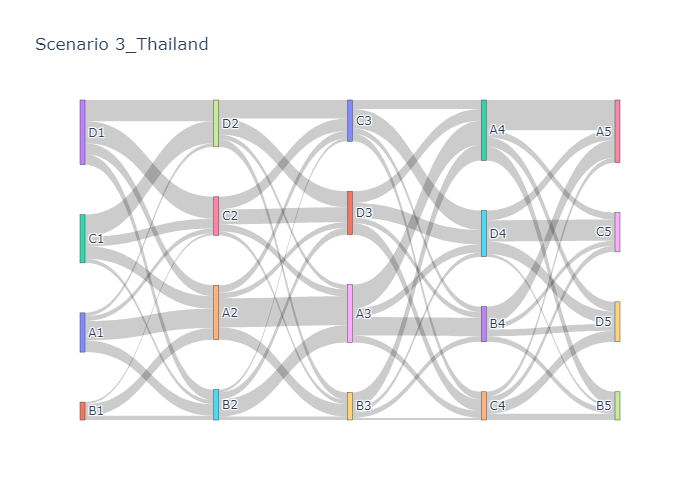
\includegraphics[width=\linewidth]{Figure/figure34c.png}
    \caption{Thailand}
  \end{subfigure}
  \begin{subfigure}{0.5\textwidth}
    \centering
    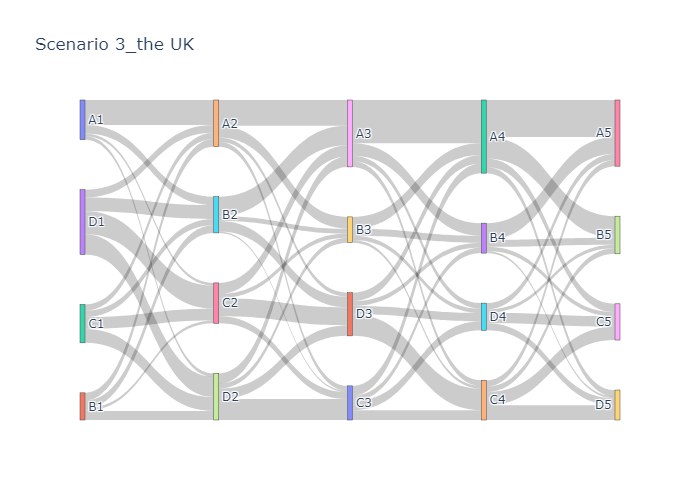
\includegraphics[width=\linewidth]{Figure/figure35c.png}
    \caption{the UK}
  \end{subfigure}
  \begin{subfigure}{0.5\textwidth}
    \centering
    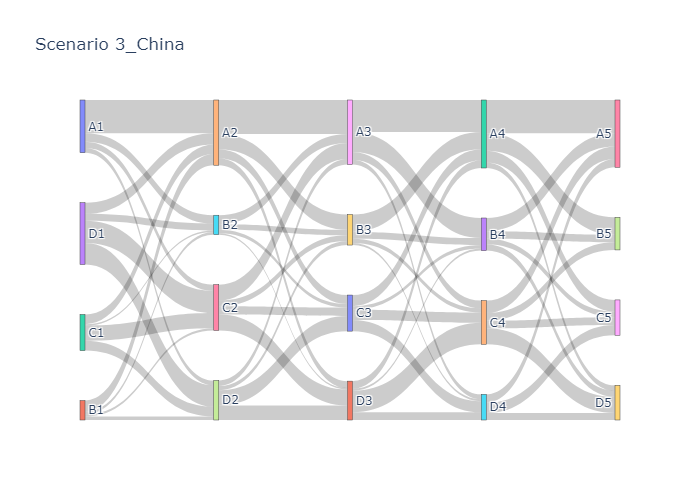
\includegraphics[width=\linewidth]{Figure/figure36c.png}
    \caption{China}
  \end{subfigure}
  \caption{ Sankey diagram of foreign vistors in senario 3 }
  \label{fig34}
\end{figure*}

\begin{figure*}[h]
  \begin{subfigure}{0.5\textwidth}
    \centering
    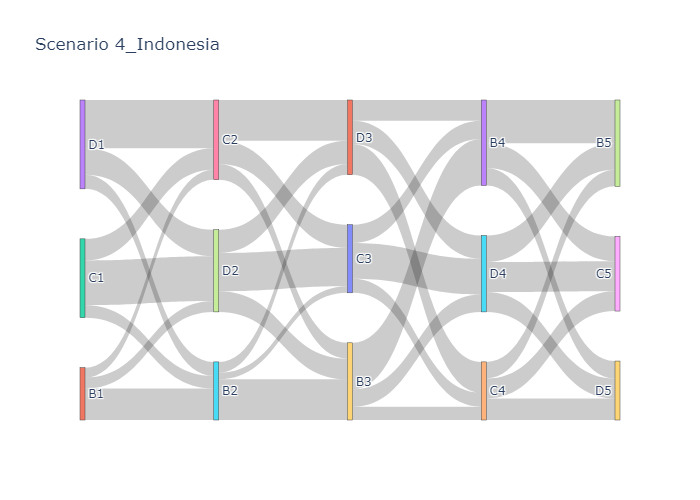
\includegraphics[width=\textwidth]{Figure/figure32d.png}
    \caption{Indonesia}
  \end{subfigure}
  \begin{subfigure}{0.5\textwidth}
    \centering
    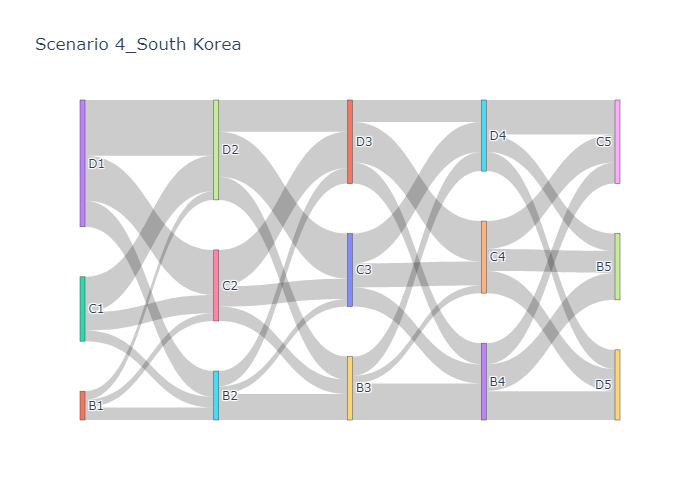
\includegraphics[width=\linewidth]{Figure/figure33d.png}
    \caption{South Korea}
  \end{subfigure}
  \begin{subfigure}{0.5\textwidth}
    \centering
    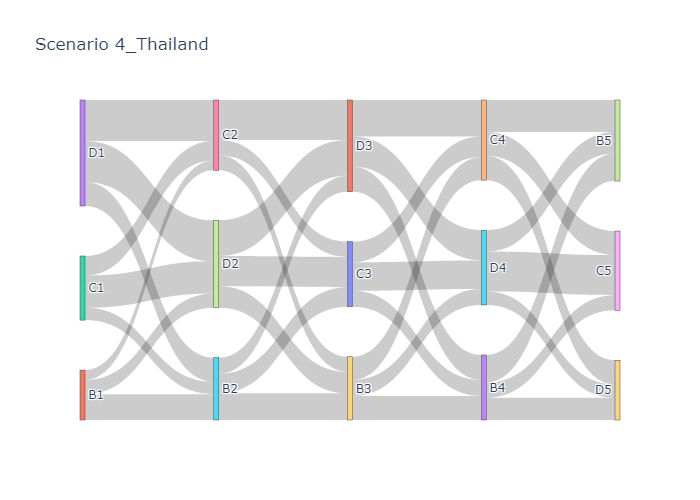
\includegraphics[width=\linewidth]{Figure/figure34d.png}
    \caption{Thailand}
  \end{subfigure}
  \begin{subfigure}{0.5\textwidth}
    \centering
    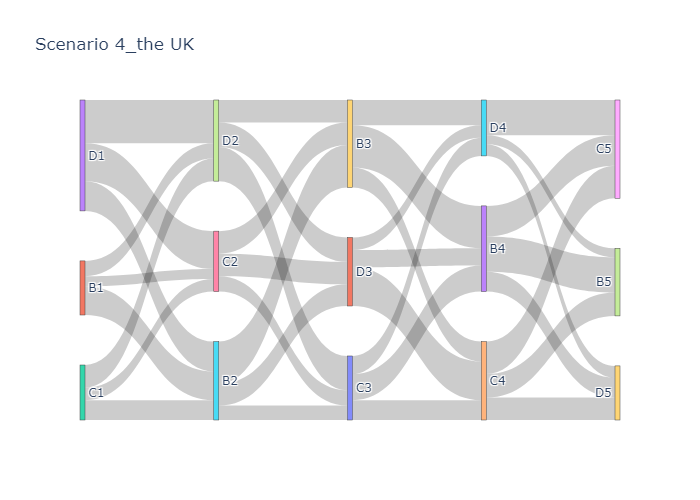
\includegraphics[width=\linewidth]{Figure/figure35d.png}
    \caption{the UK}
  \end{subfigure}
  \begin{subfigure}{0.5\textwidth}
    \centering
    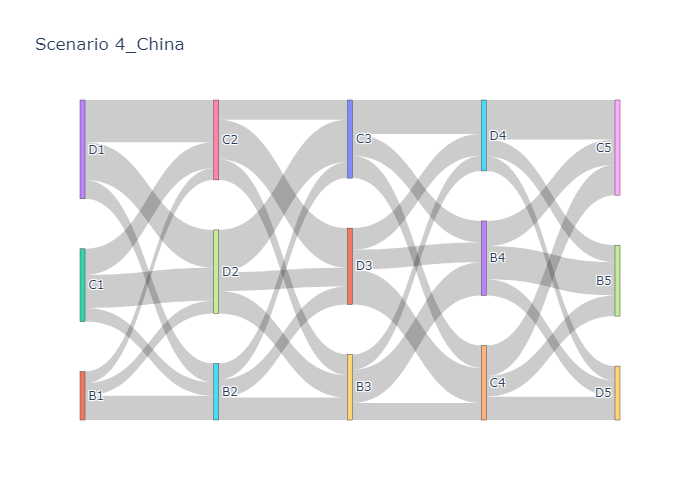
\includegraphics[width=\linewidth]{Figure/figure36d.png}
    \caption{China}
  \end{subfigure}
  \caption{ Sankey diagram of foreign vistors in senario 4 }
  \label{fig35}
\end{figure*}



















